\chapter{Kalibrering}
\mnote{Kristian Kjærgaard}

% Her beskriver vi hvordan vi kalibrerer maskinen, så højre-bredde
% forhold passer og så vi får den teoretiske maksimalhastighed

Ved kalibrering måles maskinens opløsning i $x$- og $y$-aksen og den
teoretiske topfart bestemmes.

\section{Opløsning}

Der tegnes en figur som i figur\vref{fig:kalibreringsstreg}. Stregens
retning gør, at der er mindst muligt slør til at påvirke
kalibreringen.

\mnote{
  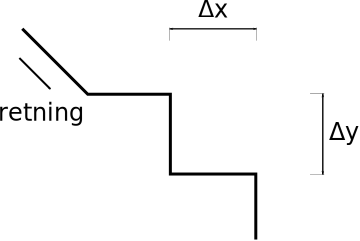
\includegraphics[width=\marginparwidth]{./img/kalibreringsstreg}
  \captionof{figure}{Streg til kalibrering}
  \label{fig:kalibreringsstreg}
}

Ved at vide hvor mange steps, der er i hver retning på stregen, kan vi
måle længden og finde $\eta_x$ og $\eta_y$ som beskrevet i
sætning\vref{eq:eta}.

Kalibrerede data fremgår af tabel\vref{tab:kalibrering}.

\begin{table}[htbp]
  \centering
  \caption{Kalibrerede data}
  \label{tab:kalibrering}
  \begin{tabular}{cc}
    \toprule
    \bfseries Symbol & \bfseries Værdi [enhed] \\
    \midrule
    $\eta_x$ & 0,297 step/gu \\
    $\eta_y$ & 1,19 step/gu \\
    \bottomrule
  \end{tabular}
\end{table}


\section{Teoretisk topfart}

Den teoretiske topfart kan bestemmes, idet vi kender opløsningen for
aksen med den højeste opløsning og den frekvens, der tjekkes
deadlines. Der kan højst flyttes ét step pr. cykle.

Vi ved, at
\begin{align}
  n_x = \frac{t_y}{\Delta t} \times \Delta x
\end{align}
og da $\Delta x = v \times \Delta t$ gælder, at
\begin{align}
  n_x &= t_x \times v \Leftrightarrow \\
  v &= \frac{n_x}{t_x} \label{eq:v-af-nxtx}
\end{align}

Formel\vref{eq:v-af-nxtx} har enheden steps pr. cykle og er lig 1, da
softwaredesignet ikke kan håndtere større hastighed.

Topfarten let omsættes til læsevenlige enheder:
\begin{align}
  v &= \frac{\SI{1}{step}}{\SI{1}{cykle}} \times \SI{1,19}{step/gu}^{-1} \\
  &= \SI{0,84}{gu/ckl} \times \SI{500}{clk/s} \\
  &= \SI{420,2}{gu/s} \times \SI{40}{gu/mm}^{-1} \\
  &= \SI{10,5}{mm/s}
\end{align}


%%% Local Variables: 
%%% mode: latex
%%% TeX-master: "../master"
%%% End: 
